\documentclass[13pt]{article}

%% Language and font encodings
\usepackage[english]{babel}
\usepackage[utf8x]{inputenc}
\usepackage[T1]{fontenc}

%% Sets page size and margins
\usepackage[a4paper,top=3cm,bottom=3cm,left=3cm,right=3cm,marginparwidth=1.75cm]{geometry}

%% Useful packages
\usepackage{amsmath}
\usepackage{graphicx}
\usepackage[colorlinks=true, allcolors=blue]{hyperref}
\usepackage{parskip}
\usepackage{subfig}
\usepackage{comment}



\title{\vspace{-2.0cm}Bayesian Spatio-Temporal approach to weather forecasting\vspace{-2ex}}
\author{\vspace{-5.0cm}Adam Pluck | Supervisor: Peter Flach}\vspace{-3ex}
\date{\vspace{-2ex}}



\begin{document}

\maketitle


\section{Project Outline}


\begin{comment}
    ever rising threat blah blah blah, hence why it is important to have good models for weather blah blah blah
\end{comment}



Classical weather forecasting methods generally consist of numerical weather prediction (NWP). This is the way in which computer simulations, in conjunction with sophisticated mathematical and physical models use the oceans and atmosphere to predict future weather conditions. These models do, however, come with an ever increasing complexity. Even with the most powerful supercomputers, "forecast skill" drops off after just the 6th day. These models are also fundamentally flawed by their intrinsic sensitivity and underlying chaotic nature further reducing efficacy as they produce further in time forecasts.

One way to overcome this is to take a data driven approach using machine learning techniques. This strategy is in its infancy when it comes to weather forecasting. Large meteorological entities such as the Met Office are, however, exploring methods such as pure Gaussian Process regression or a hybrid of both GP and NWP. These methods generally forecast for each city or region, assuming independence between each city. Although this is done with some success, particularly exceeding in the long term (6days \text{+}) forecasts, it could be argued that we are losing accuracy from that assumption. Weather features between cities are most likely correlated in some way. Hence I aim to explore the idea of taking a Bayesian Spatio-Temporal approach to weather forecasting, utilising both trends in time-series data of different weather features and also correlation in space between different locations of the United Kingdom. The ultimate goal is to produce a model that predicts precipitation in a given city using historical data from a variety of cities possibly as in Figure 1.

\begin{figure}[h]
      \centering
      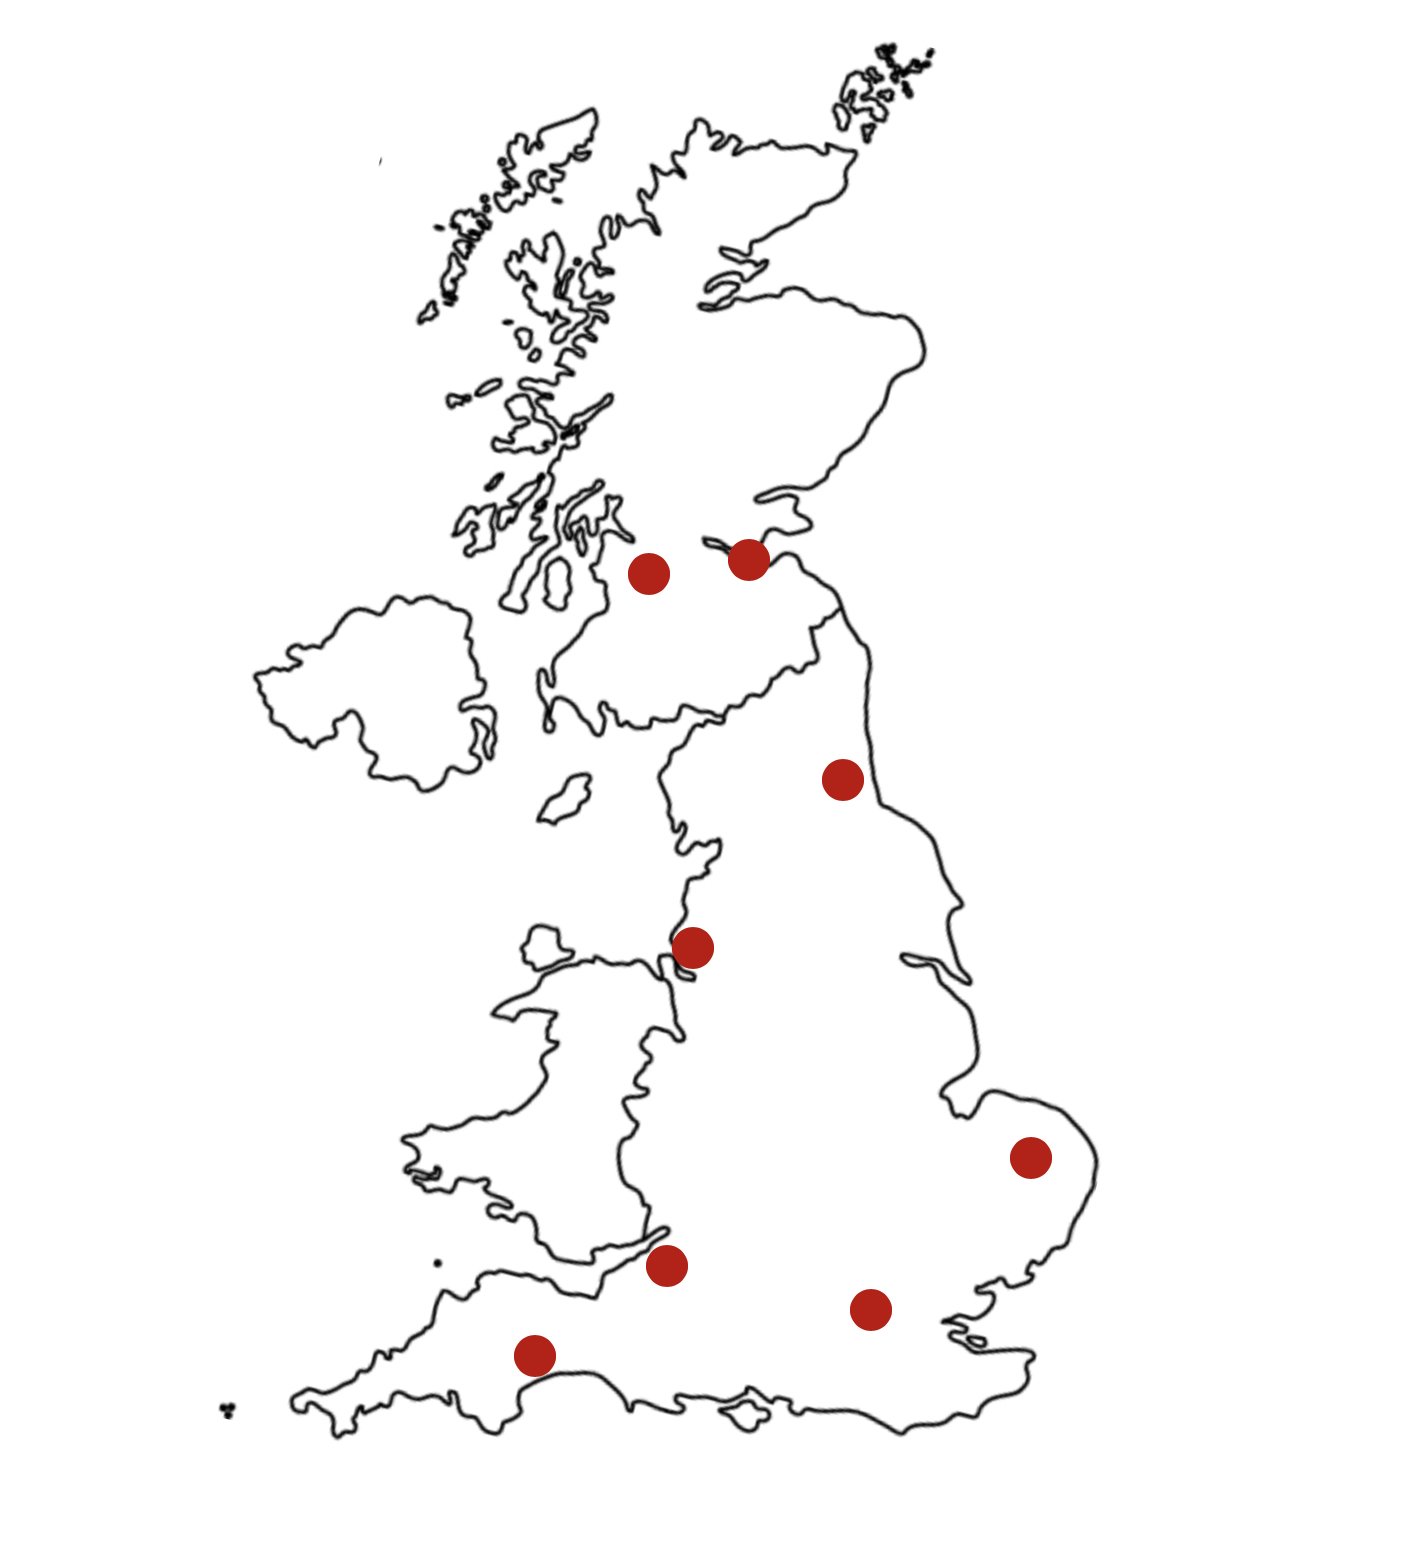
\includegraphics[width = 0.36\textwidth]{images/ukMap.png}
      \caption{Potential distribution of cities (Edinburgh, Glasgow, Newcastle, Liverpool, Norwich, Bristol, London, Exeter)}
      \label{fig:ukMap}
  \end{figure}

The data-set will be taken from the company "Dark Sky" using their own API. I will be sampling daily weather data for the past few years. Many different weather features are provided, so I will need to be careful to overcome the curse of dimentionality and reduce the number of features down to a useful amount. We also want to remove or "merge" the highly correlated features to improve the model.


\begin{comment}
    

    

Although Spatio-Temporal forecasting research is also still in its infancy with regards to weather forecasting; there has been some serious progress in the field in general. From 





My evaluation will be ... cross validation of some sort?


\clearpage{}







\section{Project Plan}

    \begin{itemize}

    \item Preface about the impact of weather on different departments (economy, agriculture, transport...) MAYBE 1 PAGEish
    
    
    \item Talk about classic weather forecasting methods 1 Page
    
    \item Talk about machine learning re forecasting 
    
    \item Talk about how spatio-temporal forecasting may work 1 page
    
    
    \item  ACTUAL PROJECT:
    \begin{itemize}
        \item Data collection, processing, feature selection
        
        
        \item ACTUAL PREDICTION MAKING THING
        
        \item Evaluation of model
    \end{itemize}
    

    \item Conclusion and evaluation of project
    
    
    \end{itemize}
    
    
    
    
    


\clearpage

Potentially Gaussian Regression for historical data at all locations, then use kriging to generate a more accurate version considering spatial data.


\section{Paper Reviews}

\subsection{Paper 1}
“Estimation and prediction of weather variables from surveillance data using spatio-temporal Kriging”\\ \url{https://upcommons.upc.edu/bitstream/handle/2117/112695/dalmau_17_kriging.pdf}

Summary of report:


\begin{itemize}


\item{}AIR TRAFFIC CONTROL
\item{}NWP = numerical weather predictions
\item{}"Kriging is a geostatistical interpolation technique to create short- term weather predictions from scattered weather observations “
\item{}Most interpolation methods estimate variable as weighted sum of observations from location  further away = lower weight
\item{}Geostatistical – data-driven statistical models that consider correlation between data e.g Kriging
\item{}Kriging interpolation provides best estimate of variable Z at unmeasured location x from set of surrounding data points


\item{}Two different methods : 
\begin{itemize}
    


\item{}do temporal regression for all cities then spatio regression to take into account the links between cities. i.e predict value for all cities, then use those values in kriging to predict a value for a single city.



\end{itemize}


\item{}Two types of spatio-temporal variogram:

\begin{itemize}


 
\item{}separable = combination of purely spatial and purely temporal variograms 
\item{}non-separable. =. “more flexible to handle…” ( above equation 17)
spatio-temporal UK (UK-ST) variant 

\end{itemize}
\end{itemize}

\subsection{Paper 2}
Improved space–time forecasting of next day ozone concentrations in the eastern US 

\url{http://www.soton.ac.uk/~sks/research/papers/sahuyipholland.pdf}


 

https://www.sciencedirect.com/science/article/pii/S2211675313000195

Spatio-temporal modeling for real-time ozone forecasting



Sahu, S.K., Yip, S., Holland, D.M., 2009a. A fast Bayesian method for updating and forecasting hourly ozone levels. Environmental 
and Ecological Statistics 18, 185–207.
Sahu, S.K., Yip, S., Holland, D.M., 2009b. Improved space–time forecasting of next day ozone concentrations in the eastern US. 
Atmospheric Environment 43, 494–501.




\subsection{Paper 3}

"A Bayesian spatio-temporal model for forecasting Anaplasma species seroprevalence in domestic dogs within the contiguous United States"

\url{https://journals.plos.org/plosone/article/file?id=10.1371/journal.pone.0182028&type=printable}

\begin{itemize}




    \item Looking at ticks in dogs across USA
    \item Show correlation between features to backup point of spatial correlation
    \item They use bayesain hierarchical spatio-temporal regression model, autocorrelated random effects are utilized to account for the spatio and temporal dependence.
    \item areal units =  places ----> use this term
    \item $Y_s(t)$ is positive test for county s at year t
    \item they have a term for "spatio-temporal random effects used to account for the spatial and temporal dependence"
    \item conditional autoregressive model (CAR) captures the spatial dependence
    \item "markov chain monte carlo posterior sampling algorithm"
    
    
    
    
    
\end{itemize}

\subsection{Paper 4}


Bowman DD, Liu Y, McMahan CS, Nordone SK, Yabsley MJ, Lund RB. Forecasting United States heartworm Dirofilaria immitis prevalence in dogs. Parasit Vectors. 2016; 9(1):540. 

\url{https://doi.org/10. 1186/s13071-016-1804-y}


\subsection{Paper 5}

"A Probabilistic Approach for Weather Forecast using Spatio-temporal Inter-relationships among Climate Variables"

\end{comment}
\end{document}